\documentclass{beamer}
\usetheme{Madrid}

\usepackage{xeCJK}
\usepackage{fontspec}
\setmainfont[
  Path = fonts/,
  UprightFont = *-Regular,
  BoldFont = *-Bold,
  ItalicFont = *-Medium,
  BoldItalicFont = *-Bold
]{NotoSansTC}
\setCJKmainfont[
  Path = fonts/,
  UprightFont = *-Regular,
  BoldFont = *-Bold,
  ItalicFont = *-Medium,
  BoldItalicFont = *-Bold
]{NotoSansTC}

\usepackage{amsmath}
\usepackage{graphicx}
\usepackage{listings}
\usepackage{xcolor}

\lstdefinestyle{cppstyle}{
  language=C++,
  basicstyle=\ttfamily\small,
  keywordstyle=\color{blue}\bfseries,
  commentstyle=\color{gray},
  stringstyle=\color{orange},
  numbers=left,
  numberstyle=\tiny\color{gray},
  stepnumber=1,
  numbersep=5pt,
  frame=single,
  breaklines=true,
  showstringspaces=false,
  tabsize=2
}

\begin{document}

\title{資料結構與演算法入門:第 1 章}
\subtitle{演算法複雜度分析}
\author{悠太翼 Yuuta Tsubasa}
\date{\today}

\frame{\titlepage}

\begin{frame}[fragile]{同樣是乘法,哪個比較快?}
\textbf{寫法一:用加法模擬乘法}
\begin{lstlisting}[style=cppstyle]
int multiply(int a, int b) {
    int result = 0;
    for (int i = 0; i < b; i++) {
        result += a;
    }
    return result;
}
\end{lstlisting}

\vspace{0.5em}
\textbf{寫法二:直接用乘法運算子}
\begin{lstlisting}[style=cppstyle]
int multiply(int a, int b) {
    return a * b;
}
\end{lstlisting}

\vspace{0.5em}
\textbf{問題:}
\begin{itemize}
    \item 如果 a = 12, b = 1000000,兩者誰比較快?為什麼?
    \item 我們可以怎麼評估程式「快不快」?
\end{itemize}
\end{frame}

\begin{frame}{各種基本運算所需的指令數(假設)}
為了更真實地比較不同程式的效率,我們先來假設:

\begin{center}
\begin{tabular}{|l|c|}
\hline
\textbf{操作類型} & \textbf{指令數(估計值)} \\
\hline
變數初始化(如 \texttt{int x = 0}) & 1 \\
加法(\texttt{x + y}) & 1 \\
乘法(\texttt{x * y}) & 2 \\
比較(\texttt{x < y}) & 1 \\
賦值(\texttt{x = y}) & 1 \\
函式呼叫(不含內容) & 1 \\
迴圈迭代一次 & 每次約 3(包含比較、執行、遞增) \\
\hline
\end{tabular}
\end{center}

\vspace{1em}
\begin{itemize}
    \item 我們會用這些估計,來推算整段程式「大概」會執行幾個基本指令
    \item 雖然實際上會更複雜,但這是理解效率的第一步
\end{itemize}
\end{frame}

\begin{frame}{怎麼比較程式的效率?}

\vspace{0.5em}
\begin{block}{加法版本的乘法:估算指令數}
\begin{itemize}
    \item \texttt{int result = 0;} → 初始化:1 指令
    \item \texttt{int i = 0;} → 初始化:1 指令
    \item \texttt{for} 迴圈跑 b 次,每次包含:
    \begin{itemize}
        \item 比較(\texttt{i < b}):1 指令
        \item 加法(\texttt{result += a}):1 指令
        \item 遞增(\texttt{i++}):1 指令
    \end{itemize}
    → 每次迴圈共 3 指令 × b 次
    \item \texttt{return result;} → 1 指令
\end{itemize}
\textbf{總共:$1 + 1 + 3b + 1 = 3b + 3$ 次指令}
\end{block}

\vspace{0.5em}
\begin{itemize}
    \item 而直接乘法如 \texttt{return a * b;} 只需約 3 指令(乘法 + return)
    \item 所以我們可以透過「基本指令總數」來估算效率差異
\end{itemize}
\end{frame}

\begin{frame}{比較兩種乘法方式的指令數}
根據我們對「基本運算所需指令數」的假設:

\begin{itemize}
    \item \textbf{方式一(用加法實作):} 總共約 $3b + 3$ 指令
    \item \textbf{方式二(直接使用乘法運算子):} 約 3 指令(乘法 + return)
\end{itemize}

\vspace{1em}
\textbf{代入不同參數來估算指令總數:}

\begin{center}
\begin{tabular}{|c|c|c|c|}
\hline
\textbf{a} & \textbf{b} & \textbf{加法實作 ($3b + 3$)} & \textbf{乘法運算子} \\
\hline
1 & 5 & 18 & 3 \\
10 & 100 & 303 & 3 \\
5000 & 6 & 21 & 3 \\
3000 & 1,000,000 & 3,000,003 & 3 \\
5 & 2,147,483,647 & 6,442,450,944 & 3 \\
\hline
\end{tabular}
\end{center}

\vspace{0.5em}
\textbf{結論:} 當輸入變大,\textbf{使用加法的版本會產生極大量的重複操作},而直接乘法始終只需常數次指令。
\end{frame}

\begin{frame}{我們想要找「上限」}
\begin{itemize}
    \item 剛才我們得到:用加法做乘法需要 $3b + 3$ 次操作
    \item 現在我們想問:
    \begin{itemize}
        \item 有沒有一個比較簡單的式子可以「估過它」?
        \item 我們不需要知道「準確」幾次,只要知道「最多大概多少」
    \end{itemize}
    \item 這就帶出「Big O」的想法!
\end{itemize}

\vspace{1em}
\begin{block}{Big O 的數學定義(非正式)}
\[
f(n) = O(g(n)) \Longrightarrow \text{存在常數 } c\text{,當 } n \text{ 很大時,}
\]
\[
\text{可以使得 } f(n) \leq c \cdot g(n)
\]
\end{block}

\vspace{0.5em}
\begin{itemize}
    \item 舉例:$3b + 3 \leq 4b$,當 $b$ 很大時就成立
    \item 所以我們說:$3b + 3 = O(b)$
\end{itemize}
\end{frame}

\begin{frame}[fragile]{從指令數推導 Big O:幾個簡單例子}
我們已經知道:可以估算每個指令的成本,  
現在我們試著從估出來的「總指令數」來找出 Big O!

\vspace{1em}
\textbf{範例一:一次加法}
\begin{lstlisting}[style=cppstyle]
int result = a + b;
\end{lstlisting}
\textbf{指令數:約 1(加法) + 1(賦值) = 2}  
→ \textbf{Big O:$O(1)$}

\vspace{0.5em}
\textbf{範例二:for 迴圈相加}
\begin{lstlisting}[style=cppstyle]
int sum = 0;
for (int i = 0; i < n; i++) {
    sum += i;
}
\end{lstlisting}
\textbf{初始:} 2 指令(sum, i)  
\textbf{每次迴圈:} 3 指令 × n  
→ \textbf{總指令數:約 $3n + 2$}  
→ \textbf{Big O:$O(n)$}
\end{frame}

\begin{frame}[fragile]{從指令數推導 Big O:巢狀迴圈}
\begin{lstlisting}[style=cppstyle]
for (int i = 0; i < n; i++) {
    for (int j = 0; j < n; j++) {
        count++;
    }
}
\end{lstlisting}

\vspace{0.1em}
\textbf{分析指令數:}
\begin{itemize}
    \item 外層:
    \begin{itemize}
        \item 初始化 \texttt{int i = 0;}:1 指令
        \item 比較 \texttt{i < n}:約 $n + 1$ 次
        \item 遞增 \texttt{i++}:約 $n$ 次
    \end{itemize}
    \item 內層(每次外層執行 n 次):
    \begin{itemize}
        \item 初始化 \texttt{int j = 0;}:$n$ 次
        \item 比較 \texttt{j < n}:$n(n + 1)$ 次
        \item 遞增 \texttt{j++}:$n^2$ 次
        \item 主體 \texttt{count++}:$n^2$ 次
    \end{itemize}
\end{itemize}

\vspace{0.1em}
\textbf{總指令數估算:約 $3n^2 + 4n + 1$}

\vspace{0.1em}
\textbf{結論:} 主導項為 $n^2$,因此這段程式的複雜度為 \fbox{$O(n^2)$}
\end{frame}

\begin{frame}{常見時間複雜度的成長速度比較}
透過 Big O 的表示法,我們可以將不同演算法的效率分門別類,  
依據「輸入大小 n 增加時,執行時間成長的快慢」來做比較。

\vspace{1em}
\begin{center}
    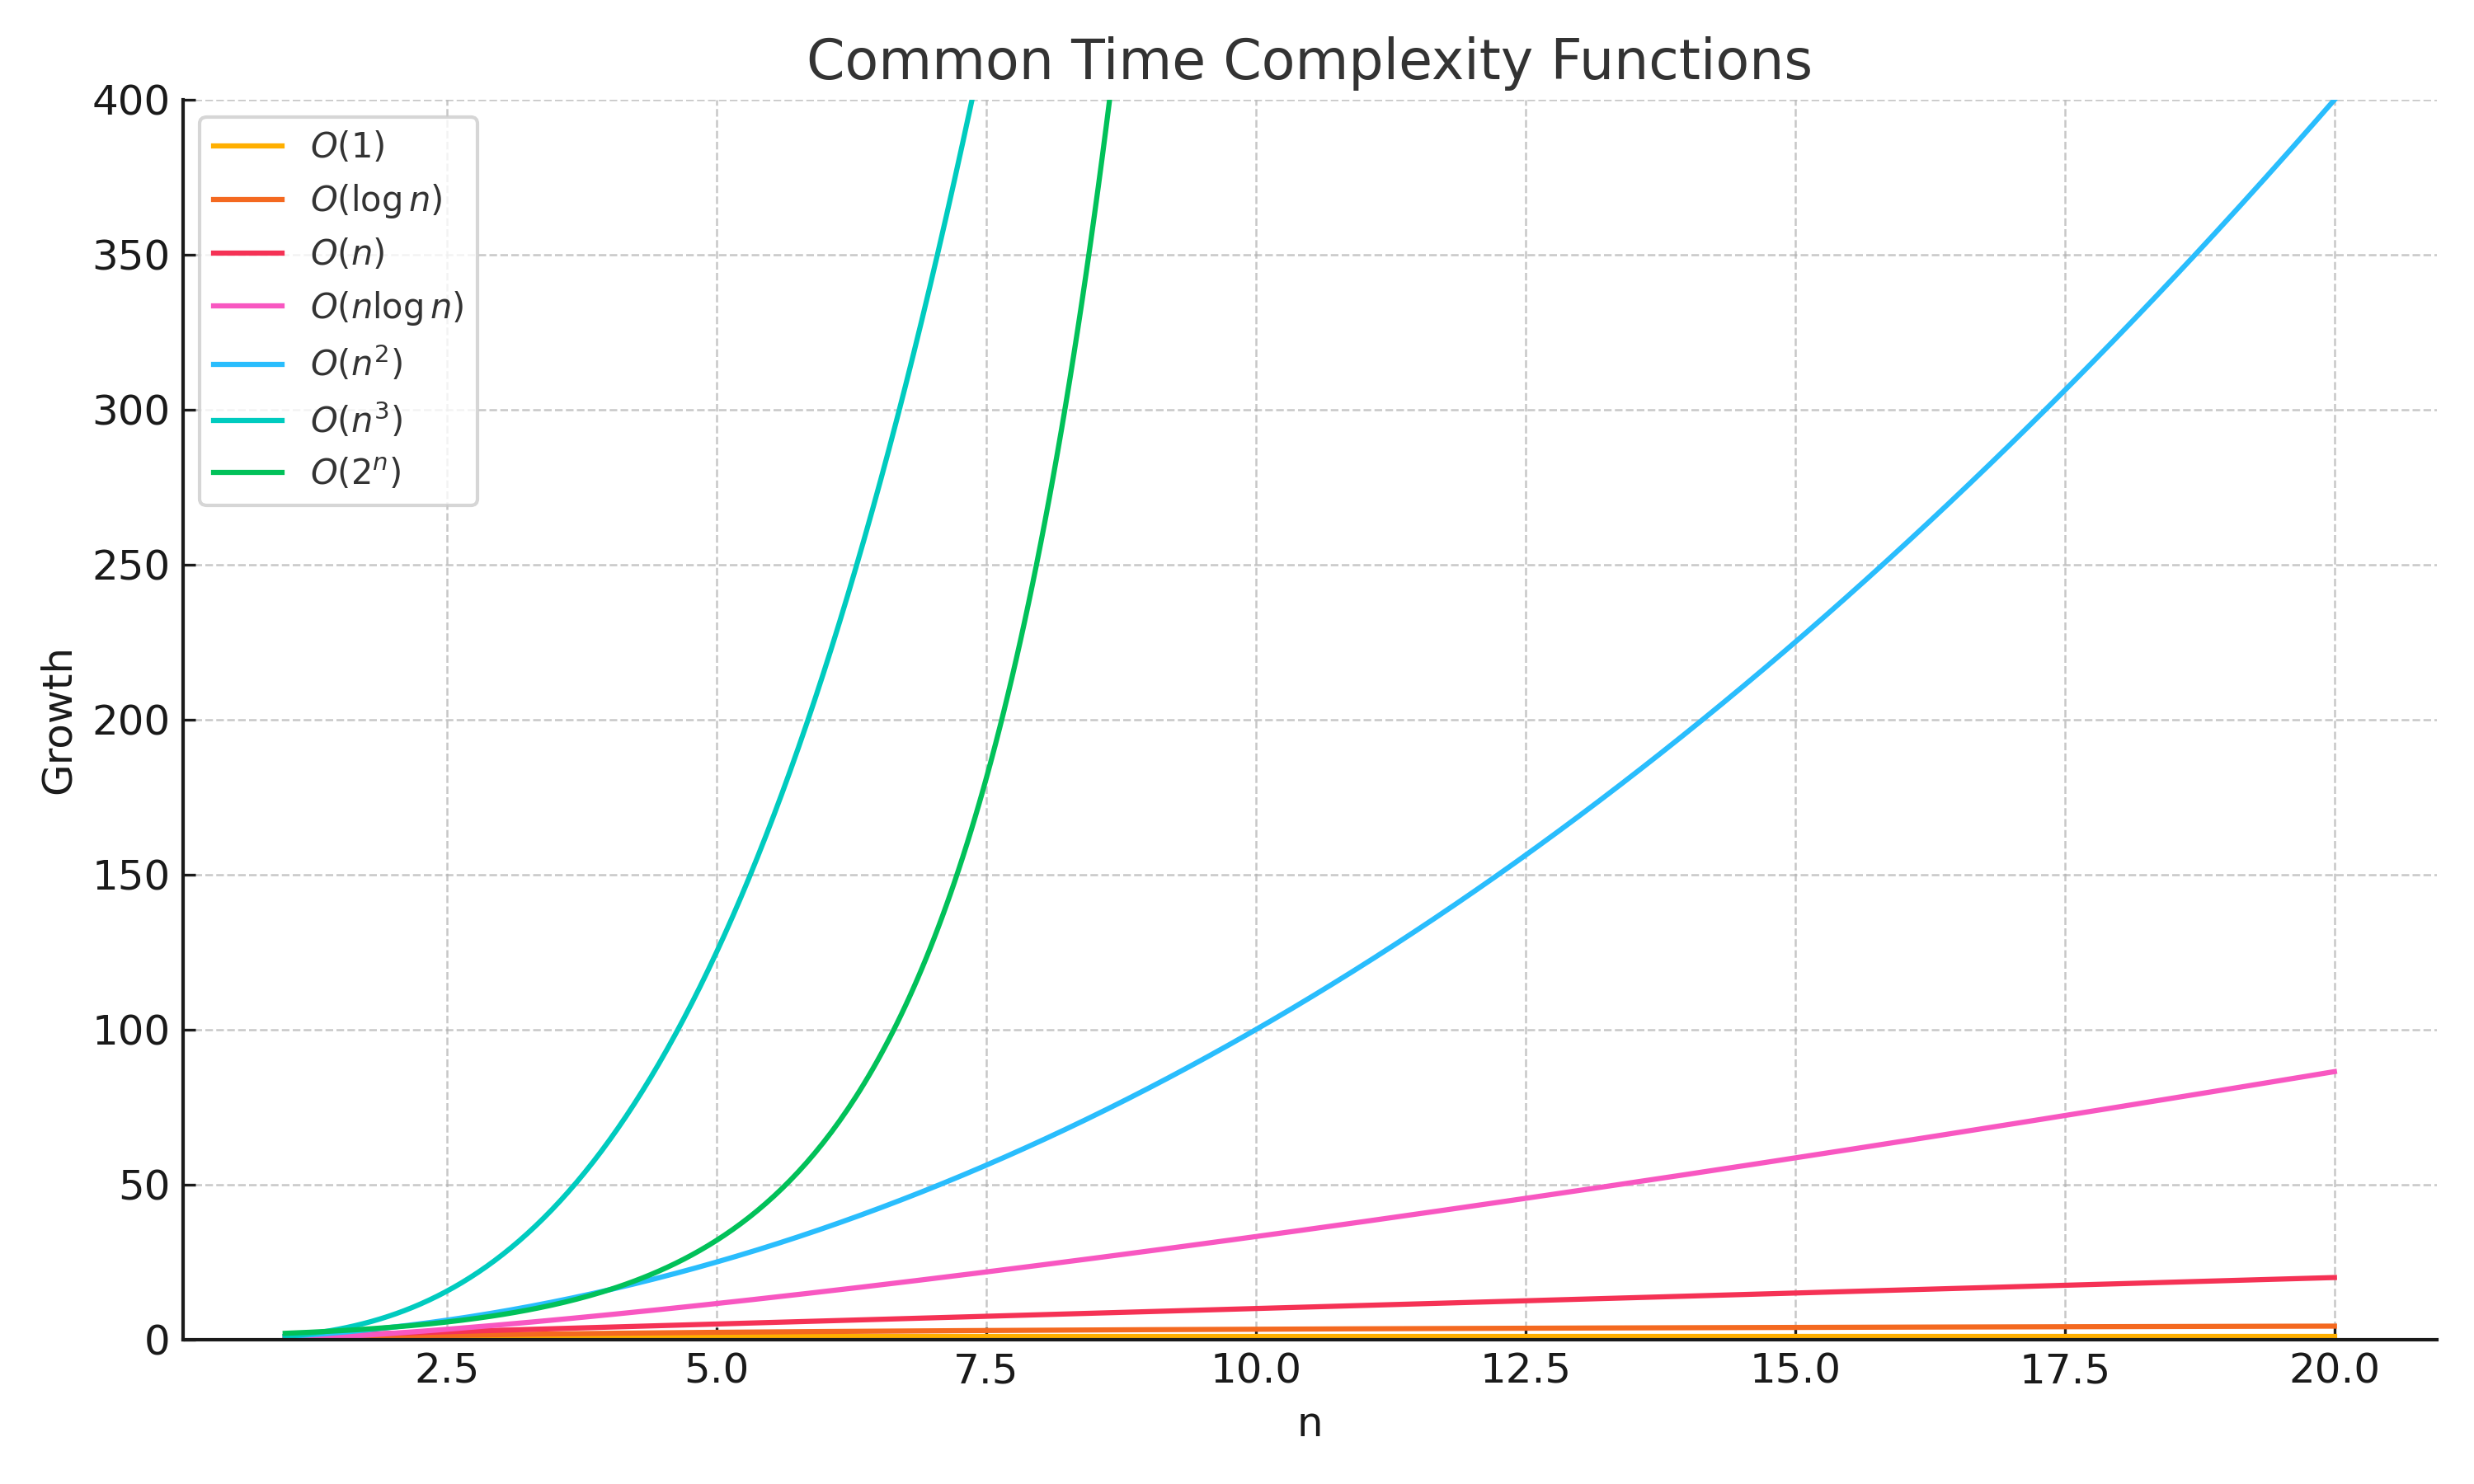
\includegraphics[width=0.9\textwidth]{images/time_complexity_curves.png}
    
    {\tiny 圖片:各種常見 Big O 成長曲線}
\end{center}

\vspace{1em}
\textbf{觀察重點:}
\begin{itemize}
    \item $O(1)$ 幾乎不變
    \item $O(n)$ 線性成長,$O(n^2)$ 明顯變慢
    \item $O(2^n)$ 成長非常快,很快就無法接受
\end{itemize}
\end{frame}

\begin{frame}{為什麼要把 n 放大來觀察?}
在前一張圖中,我們看到 $O(n^3)$ 好像比 $O(2^n)$ 還大?  
但那只是因為我們看的範圍太小,$2^n$ 的成長是「爆炸性的」,  
需要把 n 放大才能看出來!

\vspace{1em}
\begin{center}
    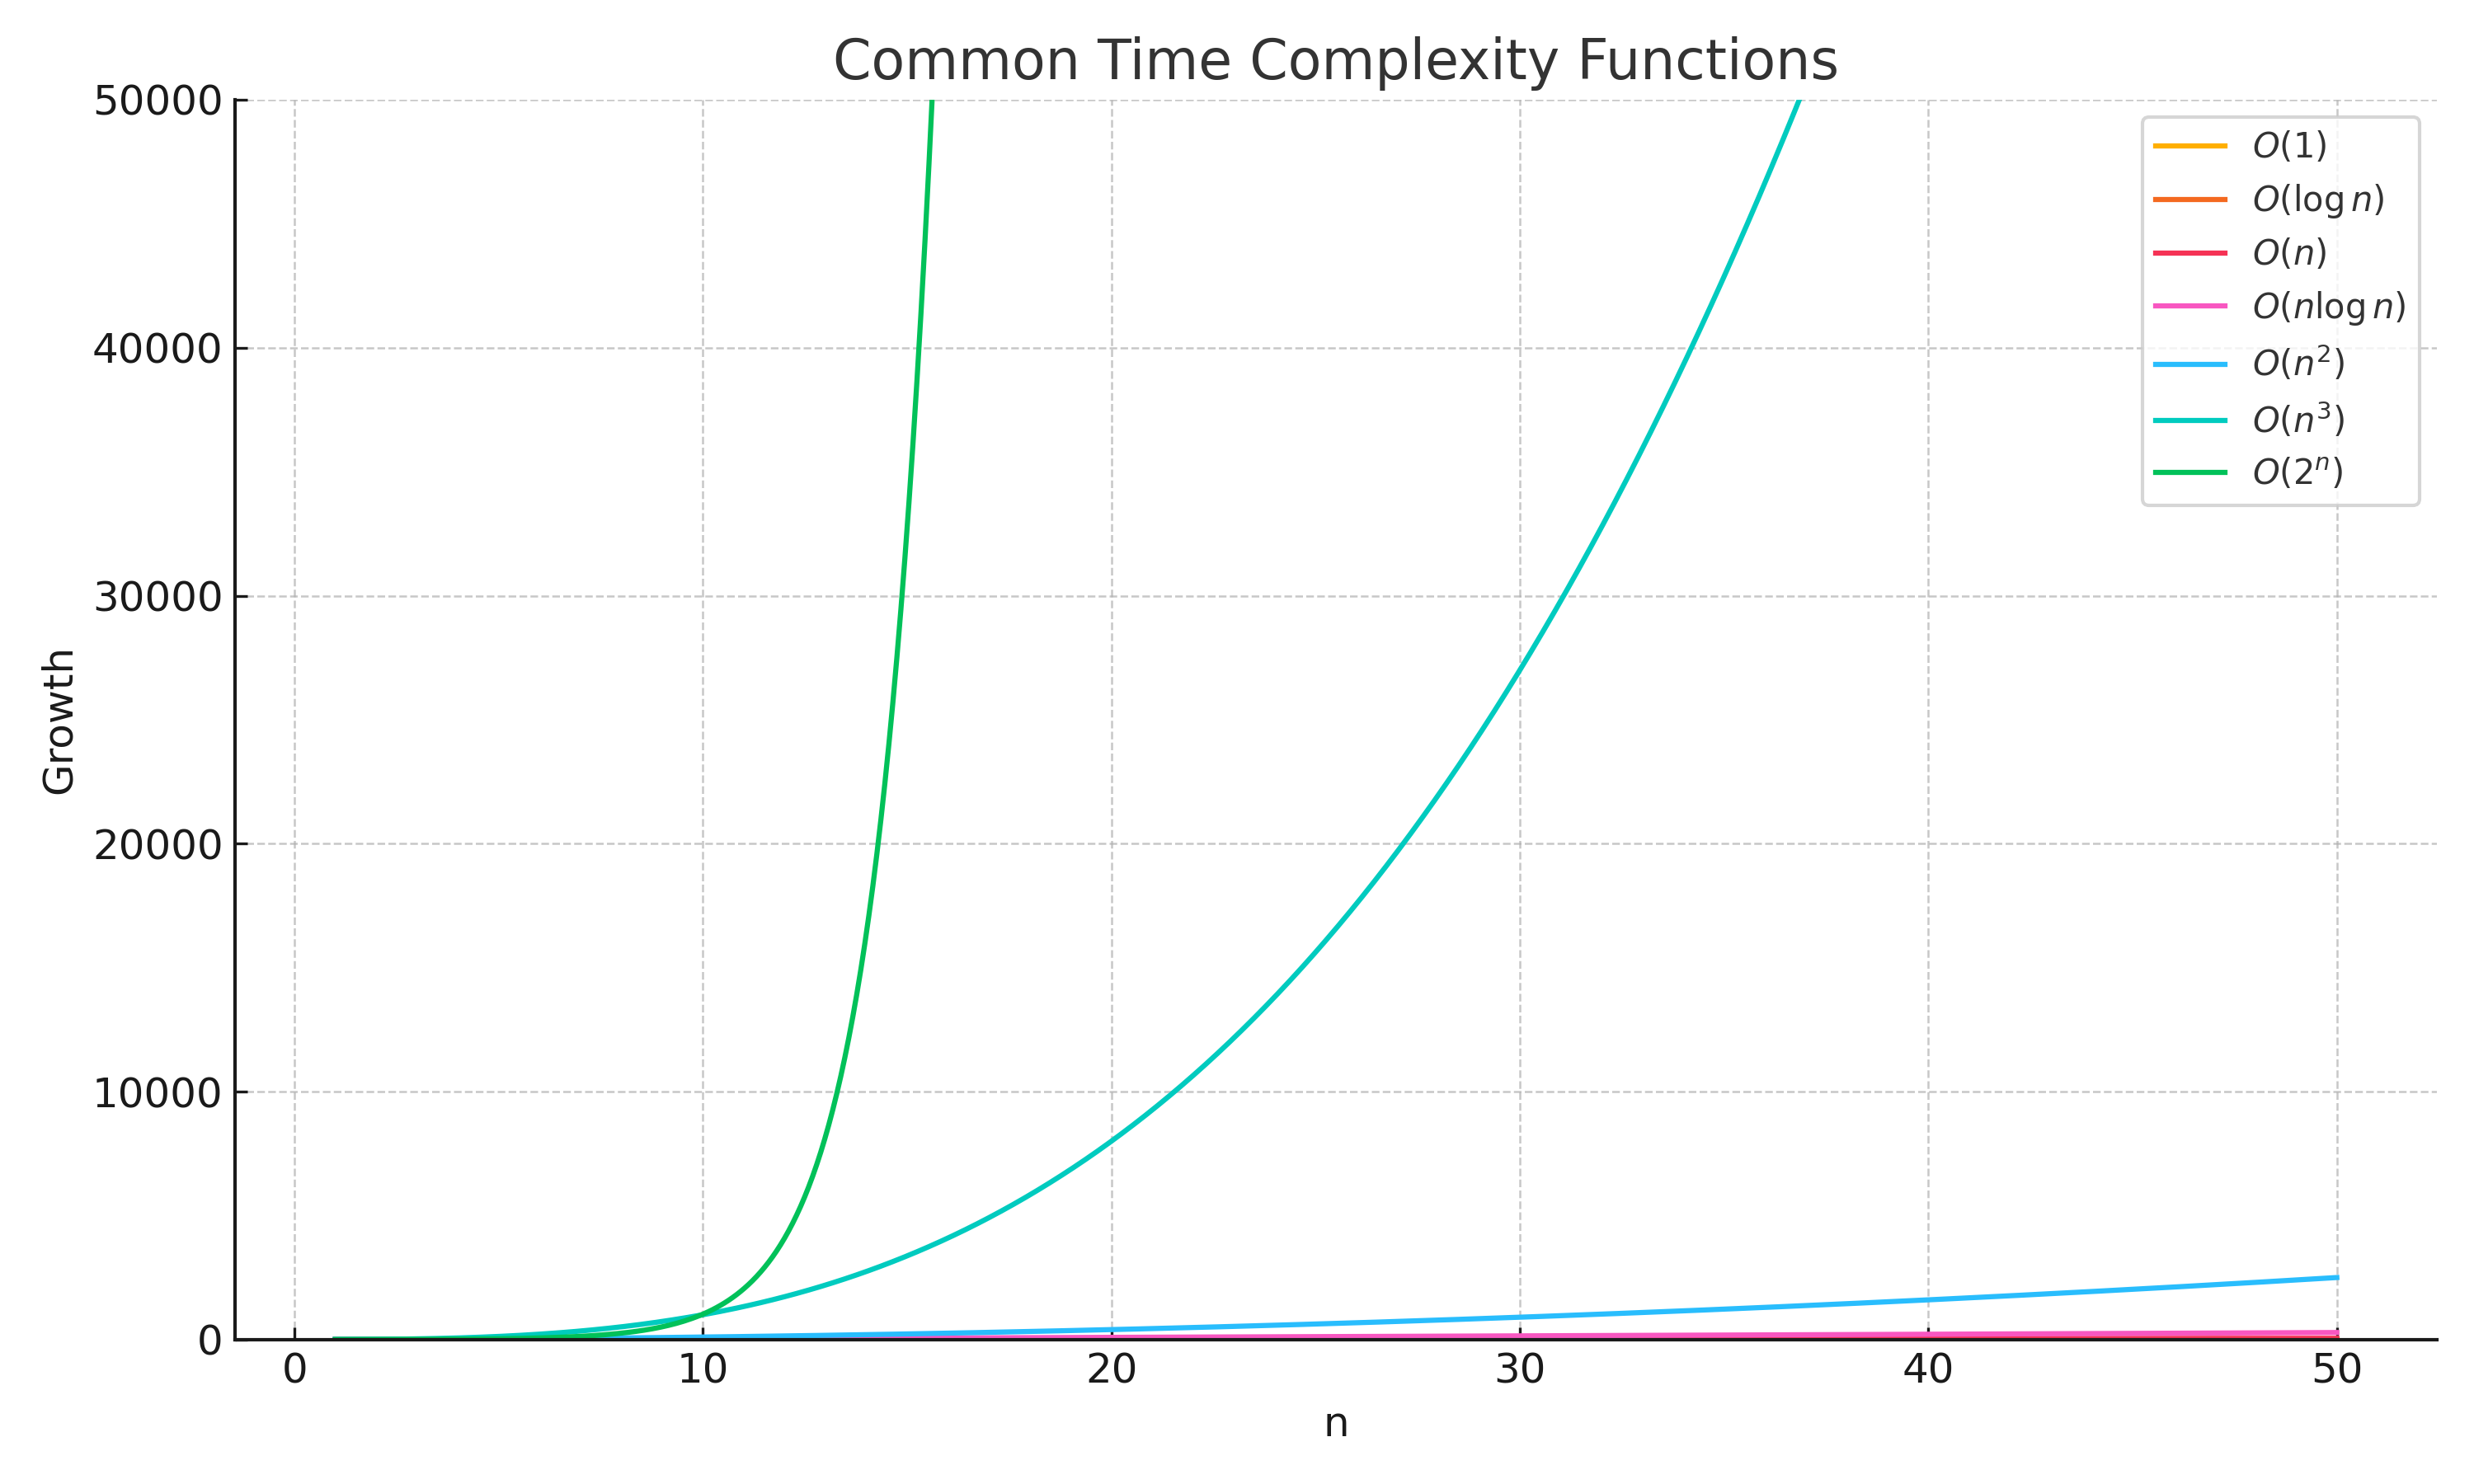
\includegraphics[width=0.9\textwidth]{images/time_complexity_curves_large_n.png}
    
    {\tiny 圖片:將 n 拉大到 50 後,可以明顯看出 $O(2^n)$ 的成長遠超過 $O(n^3)$}
\end{center}

\vspace{1em}
\textbf{結論:}
\begin{itemize}
    \item 多項式($O(n^2)$、$O(n^3)$)的成長速度仍可接受
    \item 指數級($O(2^n)$)在實務上幾乎無法處理大型輸入
\end{itemize}
\end{frame}

\begin{frame}{空間複雜度也是 Big O 的應用}
除了分析「演算法執行多久」,我們也可以分析「需要多少記憶體」  
這稱為:\textbf{空間複雜度(Space Complexity)}

\vspace{1em}
\textbf{幾個範例:}

\begin{itemize}
    \item 宣告一個變數:\quad $O(1)$ 空間
    \item 宣告一個長度為 $n$ 的陣列:\quad $O(n)$ 空間
    \item 宣告一個 $n \times n$ 的二維陣列:\quad $O(n^2)$ 空間
    \item 遞迴呼叫 $n$ 層函式,每層都有參數與區域變數:\quad $O(n)$ 空間(呼叫堆疊)
\end{itemize}

\vspace{1em}
\textbf{結論:}  
Big O 不只能用來估時間,\textbf{也可以估演算法的空間需求}
\end{frame}

\begin{frame}{進階補充:五種常見漸進符號的數學定義(可略過)}
以下是 Big O 與其他常見漸進符號的正式數學定義:

\vspace{0.1em}
\begin{center}
\renewcommand{\arraystretch}{1.5}
\begin{tabular}{|l|p{9cm}|}
\hline
\textbf{符號} & \textbf{數學定義} \\
\hline
$O(g(n))$ & 存在正實數 $c$ 和 $n_0$,使得對所有 $n \ge n_0$,都有 $f(n) \le c \cdot g(n)$ \\
\hline
$o(g(n))$ & 對所有正數 $c$,存在 $n_0$,使得對所有 $n \ge n_0$,都有 $f(n) < c \cdot g(n)$ \\
\hline
$\Omega(g(n))$ & 存在正實數 $c$ 和 $n_0$,使得對所有 $n \ge n_0$,都有 $f(n) \ge c \cdot g(n)$ \\
\hline
$\omega(g(n))$ & 對所有正數 $c$,存在 $n_0$,使得對所有 $n \ge n_0$,都有 $f(n) > c \cdot g(n)$ \\
\hline
$\Theta(g(n))$ & 同時滿足 $O(g(n))$ 與 $\Omega(g(n))$ 的條件 \\
\hline
\end{tabular}
\end{center}

\vspace{0.1em}
\textbf{備註:} 這些定義有助於理解演算法在「最佳、最壞、平均」等不同情況下的行為。
\end{frame}

\begin{frame}{本章總結}
\begin{itemize}
    \item \textbf{時間複雜度(Time Complexity)}
    \begin{itemize}
        \item 分析程式在不同輸入大小下,會執行多少「基本操作」
        \item 幫助我們預估程式的執行效率
    \end{itemize}
    
    \vspace{0.5em}
    \item \textbf{空間複雜度(Space Complexity)}
    \begin{itemize}
        \item 分析演算法需要佔用多少額外記憶體空間
        \item 特別重要於資料量龐大或遞迴深層的情況
    \end{itemize}

    \vspace{0.5em}
    \item \textbf{Big O 表示法}
    \begin{itemize}
        \item 用來描述演算法的「上限成長速度」
        \item 忽略常數與低次項,聚焦在輸入變大時的趨勢
        \item 也有 Big $\Omega$、$\Theta$ 等進階表示法
    \end{itemize}
\end{itemize}

\vspace{1em}
\begin{center}
    \textbf{搞懂這些,才是真正開始學演算法的第一步!}
\end{center}
\end{frame}

\end{document}